%%% Econ712: Macroeconomics I
%%% Fall 2020
%%% Danny Edgel
%%%
% Due on Canvas Thursday December 10th, 11:59pm Central Time
%%%

%%%
%							PREAMBLE
%%%

\documentclass{article}

%%% declare packages
\usepackage{amsmath}
\usepackage{amssymb}
\usepackage{array}
\usepackage{bm}
\usepackage{changepage}
\usepackage{centernot}
\usepackage{graphicx}
\usepackage[shortlabels]{enumitem}
\usepackage{fancyhdr}
	\fancyhf{} % sets both header and footer to nothing
	\renewcommand{\headrulewidth}{0pt}
    \rfoot{Edgel, \thepage}
    \pagestyle{fancy}
	
%%% define shortcuts for set notation
\newcommand{\N}{\mathbb{N}}
\newcommand{\Z}{\mathbb{Z}}
\newcommand{\R}{\mathbb{R}}
\newcommand{\Q}{\mathbb{Q}}
\newcommand{\lmt}{\underset{x\rightarrow\infty}{\text{lim }}}
\newcommand{\neglmt}{\underset{x\rightarrow-\infty}{\text{lim }}}
\newcommand{\zerolmt}{\underset{x\rightarrow 0}{\text{lim }}}
\newcommand{\loge}[1]{\text{ln}\left(#1\right)}
\newcommand{\usmax}[1]{\underset{#1}{\text{max }}}
\newcommand{\Mt}{M_{t+1}^t}
\newcommand{\vhat}{\hat{v}}
\newcommand{\olp}{\overline{p}}
\renewcommand{\L}{\mathcal{L}}
\newcommand{\olq}{\overline{q}}
\newcommand{\zinf}{_{t=0}^\infty}
\newcommand{\aneg}{A^{-1}}
\newcommand{\sneg}{s^{-1}}
\newcommand{\olk}{\overline{k}}
\newcommand{\olc}{\overline{c}}
\newcommand{\olr}{\overline{r}}
\newcommand{\olpi}{\overline{\pi}}
\newcommand{\Aneg}{A^{-1}}
\renewcommand{\sneg}{s^{-1}}
\newcommand{\dc}[1]{\Delta c_{#1}}

\newcommand{\E}[1]{\mathbb{E}\left[#1\right]} % expected value
\newcommand{\Et}[1]{\mathbb{E}_t\left[#1\right]}

%%% define column vector command (from Michael Nattinger)
\newcount\colveccount
\newcommand*\colvec[1]{
        \global\colveccount#1
        \begin{pmatrix}
        \colvecnext
}
\def\colvecnext#1{
        #1
        \global\advance\colveccount-1
        \ifnum\colveccount>0
                \\
                \expandafter\colvecnext
        \else
                \end{pmatrix}
        \fi
}

%%% define function for drawing matrix augmentation lines
\newcommand\aug{\fboxsep=-\fboxrule\!\!\!\fbox{\strut}\!\!\!}

\makeatletter
\let\amsmath@bigm\bigm

\renewcommand{\bigm}[1]{%
  \ifcsname fenced@\string#1\endcsname
    \expandafter\@firstoftwo
  \else
    \expandafter\@secondoftwo
  \fi
  {\expandafter\amsmath@bigm\csname fenced@\string#1\endcsname}%
  {\amsmath@bigm#1}%
}


%________________________________________________________________%

\begin{document}

\title{	Problem Set \#4 }
\author{ 	Danny Edgel 					\\ 
			Econ 712: Macroeconomics I		\\
			Fall 2020						\\
		}
\maketitle\thispagestyle{empty}

%%%________________________________________________________________%%%

\noindent\textit{Collaborated with Sarah Bass, Emily Case, Michael Nattinger, and Alex Von Hafften}

%%%________________________________________________________________%%%
\subsection*{Question 1}

\begin{enumerate}[(a)]
	\item The Bellman equation for the consumer's problem is:
		\[
			V(a,l) = \usmax{a}\left\{\frac{c^{1-\gamma}}{1-\gamma} + \beta\E{V(a',l')}\right\}\text{ s.t. } c + a' \leq wl + (1+r)a 
		\]
		Since the consumer does not value leisure, the budget constraint will hold with equality, and the Bellman becomes:
		\[
			V(a,l) = \usmax{a}\left\{\frac{(wl + (1+r)a - a')^{1-\gamma}}{1-\gamma} + \beta\int V(a',l')Q(l,dl')\right\}
		\]
		We can find the optimality conditions by taking the first order condition of the maximization problem and using the envelope condition:
		\begin{eqnarray*}
			\left(wl + (1+r)a - a'\right)^{-\gamma}(1+r) + \beta\int V'(a',l')Q(l,dl') = 0	\\
			V'(a',l') = \left(w'l' + (1+r')a' - a''\right)^{-\gamma}(-1)	\\
			\left(wl + (1+r)a - a'\right)^{-\gamma}(1+r) = \beta\E{\left(w'l' + (1+r')a' - a''\right)^{-\gamma}}
		\end{eqnarray*}
		In each period,\footnote{Since no decision made by the firm in each period affects its profits in any other period, the firm simply maximizes current-period profits each period.} the firm optimizes according to its profit-maximization problem:
		\[
			\usmax{\{K_t,N_t\}}K_t^\alpha N_t^{1-\alpha} - r_tK_t - w_tN_t
		\]
		Labor is exogenously determined by the Markov process that also governs labor for the household. Then, wages and interest rates are determined by the profit-maximizing choice of $K_t$ in each period:
		\begin{align*}
			\alpha K_t^{\alpha-1}N_t^{1-\alpha} - r_t &= 0	\\
			\Rightarrow r_t &= (N_t/K_t)^{1-\alpha}				\\
			(1-\alpha)K_t^\alpha N_t^{-\alpha} - w_t &= 0	\\
			\Rightarrow w_t &= (1-\alpha)(K_t/N_t)^\alpha
		\end{align*}
		This equilibrium either cannot be computed analytically or doing so would be prosectuable under the Geneva Conventions. We proceed computationally (see the attached Matlab code), where the final condition of the household problem becomes:
		{\tiny
		\[
			\left((1-\alpha)a^\alpha l^{1-\alpha} + (1+l^{1-\alpha})a^\alpha - a'\right)^{-\gamma}\left(1+\frac{l}{a}^{1-\alpha}\right) = 
			\beta\E{\left((1-\alpha)a'^\alpha l'^{1-\alpha} + (1+l'^{1-\alpha})a'^\alpha - a''\right)^{-\gamma}}
		\]
		}%
	
	\item 
	
	
	\item 
	
	
\end{enumerate}

%%%________________________________________________________________%%%

\subsection*{Question 2}

\begin{enumerate}[(a)]
	\item The Matlab code provided solves the Bellman equation to find the policy functions for next-period capital and current-period consumption to generate the following plots, comparing them to the deterministic model:
		\begin{center}
			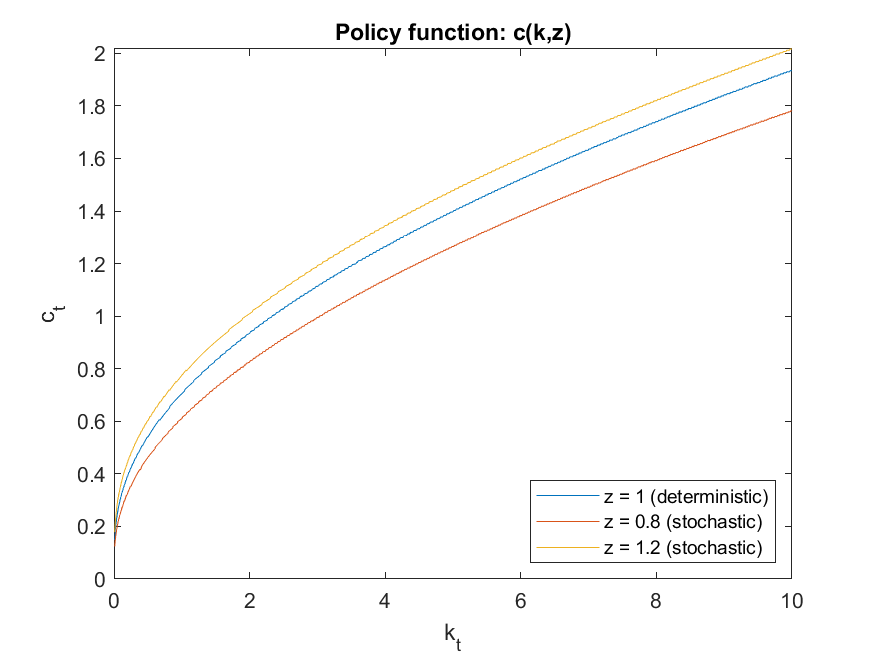
\includegraphics[scale=.75]{figure2ai.png}
		\end{center}
		\begin{center}
			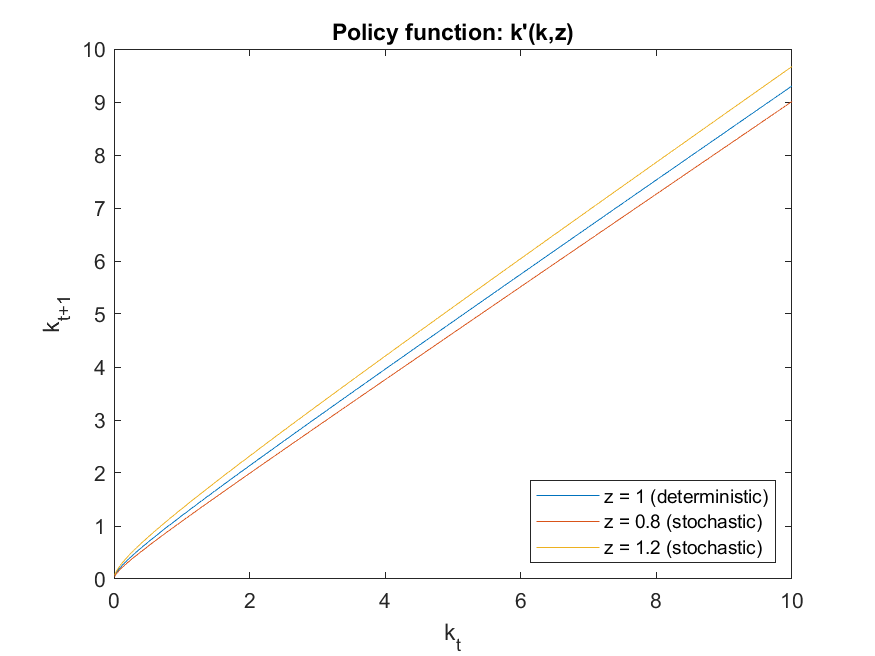
\includegraphics[scale=.75]{figure2aii.png}
		\end{center}
		As you can see, the consumer's optimal policy is to consume more in high-productivity states and less in low-productivity states, with the deterministic optimal consumption between the policy for the two states. The same is true for savings under each scenario.
	
	\item The simulated averages are displayed below, next to the steady-state values from the deterministic model. They generally track, with some noise. In general, investment is higher in the stochastic model, which is consistent with consumers building up greater capital during high-productivity periods in order to smooth consumption between the two periods.
		\begin{center}
\begin{tabular}{r c c}
& Deterministic & Stochastic \\ \hline
Capital  & 3.585 & 3.781  \\ 
Investment & 0.359 & 0.391  \\ 
Consumption & 1.205 & 1.194  \\ 
Interest rate & 0.153 & 0.154 \\ 
Wage & 1.016 & 1.030 \\ \hline
\end{tabular}
\end{center}
	
	
	\item The table below displays the standard deviation of consumption, capital, and output, respectively, along with the correlation betwen consumption and output and the correlation between interest rates and output.
		\begin{center}
\begin{tabular}{r c}
& \\ \hline
$\sigma_c$        & 0.281 \\ 
$\sigma_k$        & 1.423 \\ 
$\sigma_y$        & 0.210 \\ 
$\sigma_{c,y}$    & 0.965 \\ 
$\sigma_{r,y}$    & -0.602 \\ \hline
\end{tabular}
\end{center}
	
	
\end{enumerate}

%%%________________________________________________________________%%%

\subsection*{Question 3}
The household in this model faces the following optimization problem:
\[
	\usmax{\{c_t\}_{t=0}^\infty}\E{\sum_{t=0}^\infty \beta^tu(c_t)}\text{ s.t }c_t + k_{t+1} - (1-\delta)k_t = (1-\tau)\left(w_tN_t + r_tk_t\right) + T_t + \pi_t
\]
And the firm faces the problem:
\[
	\usmax{\{K_t,N_t\}_t=0^\infty}z_tF(K_t,N_t) - w_tN_t - r_tK_t
\]
And the government faces the following budget constraint:
\[
	T_t \leq \tau(w_tN_t + r_tk_t)
\]

\begin{enumerate}[(a)]
	\item A recursive competitive equilibrium is a continuous, bounded value function, $V(k,K,z)$ for the household; aggregate decision rules, $C(K,z)$, $N(K,z)$, ${K'=G(K,z)}$; and price rules $r(K,z)$ and $w(K,z)$ such that
		\begin{enumerate}[(i)]
			\item $V$ solves the household problem with rules $C$, $N$, and $g$
			\item Price functions $r$ and $w$ are consistent with the firm problem 
			\item Individual and aggregate behavior are consistent: ${g(k,K,z)=G(K,z)}$, ${n(k,K,z)=N(K,z)}$, ${c(k,K,z)=C(K,z)}$
			\item The government budget is balanced: ${T_t = \tau(w_tN_t + r_tk_t)}$
			\item Aggregate feasibility is satisfied: ${C(K,z) + G(K,z) - (1-\delta)K = zF(K,N(K,z))}$
		\end{enumerate}
	
	\item We begin by solving the firm's problem, which does not depend on past or future states and thus is solved in each period with a simple maximization problem with the following first-order conditions:
		\begin{align*}
			r_t &= z_tF_k(K_t,N_t)	\\
			w_t &= z_tF_N(K_t,N_t)
		\end{align*}
		We proceed by defining and solving the Bellman equation for the representative household's problem:
		\[
			V(k,K,z) = \usmax{k'}\left\{u(c) + \beta\E{V(k',K',z')|z}\right\}\text{ s.t. } c + k' = (1-\tau)\left(wN + rk\right) + T + \pi
		\]
		In equilibrium, ${T=\pi=0}$ and ${N=1}$ in all periods. We also know the distribution of $z$. Thus, we can substitute the household budget constraint for household consumption and define its optimization conditions:
		\begin{align*}
			V(k,K,z) &= \usmax{k'}\left\{u((1-\tau)\left(wN + rk\right)-k'+(1-\delta)k+T) + \beta\int V(k',K',z') P(z',z) \right\}
		\end{align*}
		\begin{align*}
			-u'(c) + \beta\int V_k(k',K',z') P(z',z) &= 0					\\
			V_k(k',K',z') &= u'(c')((1-\tau)r'+1-\delta)&\text{(Envelope condition)}	\\
			u'(c) &= \E{\beta u'(c')((1-\tau)r'+1-\delta)|z}
		\end{align*}
		Where the final optimization condition is the Euler equation that must be satisfied by the household's optimal capital accumulation policy.
	
	\item Equilibrium condition (ii) require that ${k=K}$, ${r=zf_K(K)}$, and ${w=zf_N(K)}$, where ${f(K) = F(K,1)}$. These conditions, paired with (iii), (v), and the Euler equation from (b), give us:
		\begin{align*}
			u'(C(K,z)) &= \E{\beta u'(C(K',z'))((1-\tau)zf_K(G(K,z))+1-\delta)|z}	\\
			C(K,z) + G(K,z) - (1-\delta)K &= zf(K)
		\end{align*}
		In each period, all variables in the above equations other than consumption and accumulated capital are given. Thus, we have two equations and two unknowns and the above serves as a functional equation that the aggregate capital accumulation policy must satisty.
	
	\item If ${\delta=1}$, then our aggregate feasibility constraint is ${C(K,z) + G(K,z) = zf(K)}$ and the household's budget constraint in each period\footnote{Assuming zero profits} is ${c + k' = (1-\tau)\left(wN + rk\right) +T}$. Then, our functional equation is:
		\begin{align*}
			u'(C(K,z)) &= \E{\beta u'(C(K',z'))((1-\tau)z'f_K(G(K,z)))|z}	\\
			C(K,z) + G(K,z) &= zf(K)
		\end{align*}
		The social planner's problem in this model is:
		\[
			\usmax{\{c_t\}_{t=0}^\infty}\E{\sum_{t=0}^\infty \beta^tu(c_t)}\text{ s.t } c_t + k_{t+1} = z_tF(K_t,N_t)
		\]
		Where, letting ${N_t=1}$ for all $t$ and substituting the feasibility constraint, the planner's Bellman equation is:
		\[
			V(K,z) = \usmax{k'}\left\{u(zF(k)-k') + \beta\E{V(K',z')|z}\right\}
		\]
		With the following optimization condition (and Euler equation):
		\[
			u'(c) = \E{\beta u'(c')(z'f_k(k')|z}	
		\]
		Thus, when ${\delta=1}$, the social planner's problem and competitive equilibrium have the same feasibility condition, with the following Euler equations:
		\begin{align*}
			u'(c) &= \E{\beta(1-\tau)z'f_k(k')u'(c')|z}	&\text{(CE)}	\\
			u'(c) &= \E{\beta z'f_k(k') u'(c')|z}		&\text{(SPP)}
		\end{align*}
		So the competitive equilibrium's allocation is equal to the social planner's allocation if the social planner optimized using a discount factor that's multiplied by ${1-\tau}$. The interpretation of this result is that a tax, equally applied to all income and redistributed as a lump-sum payment, distorts the competitive equilibrium by lowering the value that agents place on future consumption (i.e. by making them more impatient).
	
\end{enumerate}


%%%________________________________________________________________%%%

\subsection*{Question 4}

\begin{enumerate}[(a)]
	\item 
	
	
	\item 
	
	
	\item 
	
	
\end{enumerate}

\begin{enumerate}[(a)]
	\item 
	
	
	\item 
	
	
	\item 
	
	
	\item 
	
	
	\item 
	
	
\end{enumerate}

%%%________________________________________________________________%%%


\end{document}







